\documentclass{willowtreebook}
\usepackage{url}
\usepackage{tikz}
\usepackage{quiver}
\usetikzlibrary{shapes}
\usetikzlibrary{decorations.pathreplacing}
\colorlet{lgray}{gray!25}
\colorlet{llgray}{gray!50}
\usepackage{tikz-cd}
\usepackage{cleveref}

\newcommand{\nc}{\newcommand}
\nc{\ul}{\underline}
\nc{\dmo}{\DeclareMathOperator}
\dmo{\Sub}{Sub}
\nc{\bbZ}{\mathbb{Z}}
\nc{\bbR}{\mathbb{R}}
\nc{\bbC}{\mathbb{C}}
\nc{\cat}[1]{\mathscr{#1}}
\nc{\Mid}{\,\big|\,}
\nc{\normal}{\trianglelefteq}
\nc{\SET}[2]{\big\{\,#1\Mid#2\,\big\}}

\dmo{\Mack}{Mack}
\dmo{\FinSet}{Fin}
\dmo{\End}{End}
\dmo{\Top}{Top}
\dmo{\Inf}{Inf}
\dmo{\ev}{ev}
\dmo{\Conj}{Conj}
\dmo{\Mod}{Mod}
\dmo{\Res}{Res}
\dmo{\Ind}{Ind}
\dmo{\Coind}{Coind}
\dmo{\Grp}{Grp}
\dmo{\Aut}{Aut}
\dmo{\Iso}{Iso}
\dmo{\Map}{Map}
\dmo{\sgn}{sgn}
\dmo{\Hom}{Hom}
\dmo{\id}{id}
%%Alternative command for C_p-Lewis diagrams
\newcommand{\lew}[5]{
\begin{tikzcd}
    #1 \arrow[d, "#3", curve={height=3pt}, swap, shift right=2] \\
    #2 \arrow[u, "#4", swap, curve={height=3pt}, shift right=2] \arrow[loop, "#5", distance=20, out=300,in=240]
\end{tikzcd}
}

\Crefname{example}{Example}{Examples}
\Title{MA8403  - Equivariant homotopy theory}
\Author{Drew Heard}
\BibliographyFile{ma8403} 		
	% The name of the .bib file, without file extension.
\begin{document}
\chapter{Preface}
This are the courses notes for MA8403 - Equivariant homotopy theory, held during the Autumn semester 2023 at NTNU. The notes are mainly based on two excellent sets of lectures notes, one by Guillou \cite{guillou}, and one by Blumberg \cite{blumberg}. The notes will be continually updated during the semester. 
\afterpreface
\chapter{Equivariance in algebra}
\subsection{Group actions in algebra}
We recall that if $X$ is an object in a category $\cat C$, then the set of endomorphisms $\End(X)$ forms a monoid (that is, a set equipped with an associative binary operation and an identity element) under composition. The set of automorphisms of $X$ (that is, those endomorphisms that are invertible) form a group. Moreover, we have
\[
\Aut(X) = \End(X) \cap \Iso(\cat C)
\]

Note that any group is a monoid, simply by forgetting the existence of inverses. 
\begin{definition}\label{def:group-action}
    An action of a group $G$ on an object $X \in \cat C$ is a monoid homomorphism $a \colon G \to \End(X)$, or equivalently a group homomorphism $a \colon G \to \Aut(X)$ (note that a monoid homomorphism between groups is a group homomorphism). 
\end{definition}
\begin{remark}
    Unwinding the definition, this means that we have:
    \begin{enumerate}
        \item For each $g \in G$, there is a morphism $a(g) \colon G \to G$.
        \item $a$ preserves composition, i.e., $a(g \cdot h) = a(h) \cdot a(h)$. 
        \item $a$ preserves identifies, so $a(e) = \id_X$.
    \end{enumerate}
\end{remark}
\begin{example}
    Let $\cat C$ be the category of sets and functions. Then, $a \colon G \to \End(X) = \big\{\,f \colon X \to X\big\}$ correspond to a function $\overline{a} \colon G \times X \to X$. The conditions above mean that the diagrams
    % https://q.uiver.app/#q=WzAsNCxbMCwwLCJHIFxcdGltZXMgRyBcXHRpbWVzIFgiXSxbMCwxLCJHIFxcdGltZXMgWCJdLFsxLDAsIkcgXFx0aW1lcyBYIl0sWzEsMSwiWCJdLFswLDEsIlxcaWQgXFx0aW1lcyBcXG92ZXJsaW5le2F9IiwyXSxbMCwyLCJtIFxcdGltZXMgXFxpZCJdLFsyLDMsIlxcb3ZlcmxpbmV7YX0iXSxbMSwzLCJcXG92ZXJsaW5le2F9IiwyXV0=
\[\begin{tikzcd}[ampersand replacement=\&]
	{G \times G \times X} \& {G \times X} \\
	{G \times X} \& X
	\arrow["{\id \times \overline{a}}"', from=1-1, to=2-1]
	\arrow["{m \times \id}", from=1-1, to=1-2]
	\arrow["{\overline{a}}", from=1-2, to=2-2]
	\arrow["{\overline{a}}"', from=2-1, to=2-2]
\end{tikzcd}
\text{ and }
% https://q.uiver.app/#q=WzAsNCxbMCwwLCJcXHtcXGFzdFxcfSBcXHRpbWVzIFgiXSxbMSwwLCJHIFxcdGltZXMgWCJdLFswLDEsIlgiXSxbMSwxLCJYIl0sWzAsMSwiZSBcXHRpbWVzIFxcaWQiXSxbMCwyLCJcXGNvbmciLDJdLFsxLDMsIlxcb3ZlcmxpbmV7YX0iXSxbMiwzLCIiLDIseyJsZXZlbCI6Miwic3R5bGUiOnsiaGVhZCI6eyJuYW1lIjoibm9uZSJ9fX1dXQ==
\begin{tikzcd}[ampersand replacement=\&]
	{\{\ast\} \times X} \& {G \times X} \\
	X \& X
	\arrow["{e \times \id}", from=1-1, to=1-2]
	\arrow["\cong"', from=1-1, to=2-1]
	\arrow["{\overline{a}}", from=1-2, to=2-2]
	\arrow[Rightarrow, no head, from=2-1, to=2-2]
\end{tikzcd}\]
commute, where $m \colon G \times G \to G$ denotes the group multiplication. Equivalently, in symbols, we have
\[
\overline{a}(h,\overline{a}(h,x)) = \overline{a}(gh,x) 
\]
and
\[
\overline{a}(e,x) = x. 
\]
\end{example}
\begin{remark}
    Let $BG$ denote the category with one object $\ast$ and with $\Hom(\ast,\ast) = G$. Then an action of $G$ in the category $\cat C$ is the same as a functor $\rho \colon BG \to \cat C$. The object $X$ in the previous definition is the object $\rho(\ast) \in \cat C$. 
\end{remark}
\begin{remark}
    Let $\cat C = \Mod_R$ for a commutative ring $R$. An action of $G$ on $M \in \Mod_R$ is a monoid homomorphism
    \[
a \colon G \to \Hom_R(M,M).
    \]
    We recall that $\Hom_R(M,M)$ actually has the structure of an $R$-algebra
\end{remark}
\begin{definition}
    The ($R$-linear) group ring on $R$ is the $R$-algebra $R[G]$ whose:
    \begin{enumerate}[label=(\alph*)]
    \item underlying $R$-module is the free $R$-module with basis on the underlying set of $G$. 
    \item whose multiplication is given on basis elements by the group operation. 
    \end{enumerate}
\end{definition}
\begin{example}
    Let $R = \mathbb{Z}$ and $G = C_2 = \langle \sigma \rangle$. An element of $\bbZ[C_2]$ is of the form $a + b\sigma$ where $a,b \in \bbZ$. Multiplication is given by
    \[
(a_1 \cdot 1+b_1\sigma)\cdot(a_2\cdot 1+b_2\sigma) = (a_1a_2+b_1b_2)\cdot 1  + (a_1b_2+b_1a_2)\sigma. 
    \]
    This is the same thing as the polynomial ring $\bbZ[\sigma]/(\sigma^2-1)$. 
\end{example}
\begin{remark}
    Categorically, the group ring construction is left adjoint to the functor that takes an $R$-algebra to its group of units, i.e., there is an adjudication
    \[
R[-] \colon \Grp \leftrightarrows \Mod_R \colon (-)^{
\times}
    \]
\end{remark}
Returning to group actions, we have the following:
\begin{proposition}
    Let $R$ be a commutative ring, and $G$ a finite group. The following data on an $R$-module $M$ are equivalent:
    \begin{enumerate}
        \item A monoid homomorphism $G \to \End_R(M)$.
        \item A group homomorphism $G \to \Aut_R(M)$. 
        \item A homomorphism of $R$-algebras $R[G] \to \Hom_R(M,M)$. 
        \item An $R[G]$-module structure on $M$ whose underlying $R$-module structure is $M$. 
    \end{enumerate}
\end{proposition}
\begin{definition}
    A representation of $G$ over $R$ is an $R[G]$-module. 
\end{definition}
\begin{example}
    If $R = k$ is a field, then the underlying $R$-module is a $k$-vector space $V$. If $\dim_k(V) = n$, then $\Aut_k(V) = GL_n(k)$, and a $k$-representation is the same thing as a group homomorphism $G \to GL_n(k)$. 
\end{example}
\begin{definition}
    The $R[G]$-module $R[G]$ is known as the regular representation. More generally, if $X$ is a finite $G$-set, then the free $R$-module $R[X]$ inherits the structure of a $R[G]$-module (the case of $R[G]$ itself corresponds to the finite $G$-set $G$, considered as an $R[G]$-module over itself). Representations obtained this way are known as permutation representations. 
\end{definition}
\begin{example}
    Taking $X$ to be the trivial $G$-set, we obtain the (one-dimensional) trivial representation. This is simply the $R[G]$-module $R$, where $G$ acts trivially. 
\end{example}
\begin{definition}
    Let $G = C_2 = \langle \tau \rangle$, and suppose that $-1 \ne 1 \in R$. Then the sign representation of $G$ is the one-dimensional representation where $\tau$ acts as $-1$ (if $-1 = 1$ in $R$ this still makes sense, but is just the trivial representation). Note that this is an example of a representation that is not a permutation representation.
\end{definition}
\begin{example}
    Let $C_n = \langle \sigma \rangle$ be the cyclic group of order $n$. Let us calculate all complex 1-dimensional representations of $C_n$, i.e., homomorphisms $\rho \colon C_n \to \mathbb{C}$. Note that if we define $\rho(\sigma) =c$, then $\rho(\sigma^n) = c^n = 1$, so that $c$ must be an $n$-th root of unity. There are precisely $n$-of these (take $\zeta_n = e^{2\pi/n i}$), and so there are precisely $n$-representations. For example, when $G = C_4$, the four representations correspond to sending $\sigma$ to either $1,i,-1$ or $-i$. Note that we can also consider these as 2-dimensional \emph{real} representations. 
\end{example}
\begin{notation}
We let $\rho = \rho_G$ denote the regular representation of $G$, and the trivial $n$-dimensional representation by $\mathbf{n} = R^{\oplus n}$. 
\end{notation}
\begin{definition}
    A subrepresentation is a submodule. 
\end{definition}
\begin{example}
    The regular representation always has a one-dimensional trivial representation, generated by the sum $\sum_{g \in G}g$. 
\end{example}
\begin{definition}
    A representation $V$ is irreducible if the only subrepresentations of $V$ are $0$ and $V$. 
\end{definition}
\begin{theorem}[Maschke]Suppose that $k$ is a field of characteristic not dividing $|G|$. Then every
representation splits as a direct sum of irreducible representations.
\end{theorem}
\begin{proof}
    We prove the following: if $V \subseteq W$ is a subrepresentation, then there exists $U \subseteq W$ such that $U \oplus V \simeq W$. 

    To see this, let $\pi \colon W \to W$ be any $k$-linear projection of $W$ onto $V$. This map need not be $G$-equivariant, but we can make it so by `averaging'. That is, we define a new map $\phi \colon W \to W$ by 
    \[
\phi(\mathbf{w}) = \frac{1}{|G|}\sum_{g \in G}g \cdot \pi(g^{-1} \cdot \mathbf{w}). 
    \]
   Moreover the map is $G$-equivariant: for $h \in G$ we have
   \[
   \begin{split}
\phi(h \cdot \mathbf{w}) &= \frac{1}{|G|}\sum_{g \in G}g \cdot \pi(g^{-1} \cdot h \cdot \mathbf{w}) \\
& = \frac{1}{|G|}\sum_{u \in G}u \cdot h \cdot \pi(u^{-1} \cdot \mathbf{w}) \\
&= h \cdot \phi(\mathbf{w}),
\end{split}
   \]
   where $u = gh^{-1}$, and so $\phi$ is $k[G]$-linear. Furthermore, the map $\phi$ is the identity on $V$ By the splitting lemma, $W = V \oplus \ker(\phi)$. 
\end{proof}
\begin{remark}
We used the assumption on $k$ to ensure that we could divide by $|G|$. Without that assumption, the theorem is false. Indeed, let $G = C_2$, $R = \mathbb{F}_2$ and consider the representation defined by $\rho(\tau) =\begin{pmatrix}
1 & 1 \\
1 & 0 
\end{pmatrix} $. This is not irreducible, but does not split as a direct sum of indecomposable representations. 
\end{remark}
\begin{corollary}
Suppose that $k$ is a field of characteristic not dividing $|G|$.  If $V$ is an irreducible representation, then $V$ is isomorphism to a subgroup of $k[G]$ (slogan: all irreducibles are submodules of the regular representation). 
\end{corollary}
\begin{proof}
    Let $\mathbf{v} \in V$ be non-trivial. Then the homomorphism $\phi \colon k[G] \to V$ given by sending $1$ to $\mathbf{v}$ must be surjective, because $V$ is irreducible. Let $U = \ker(\phi)$, then apply Maschke's theorem. 
\end{proof}
\begin{example}
    Let $G = C_2 = \langle \tau \rangle$, and $k$ a field of characteristic not equal to 2. We have the trivial representation $\mathbf{1}$ and the sign representation $\mathbf{1}_{\sgn}$. Then, $\mathbf{1}$ is generated by the sum $1+\tau$, while $\mathbf{1}_{\sgn}$ is generated by $1-\tau$, and we deduce that 
    \[
\rho_{C_2} = \mathbf{1} \oplus \mathbf{1}_{\sgn}. 
    \]
\end{example}
\section{The representation ring}
Let $k$ be a field, and suppose that $V$ and $W$ are $G$-representations, then the $k$-linear tensor sum $V \oplus W$ can be given the structure of a $k[G]$-module, by taking the diagonal $G$-action. If we think of a representation in terms of a homomorphism $\rho \colon G \to GL_n(k)$, then this direct sum corresponds to the `block sum'
\[
G \to GL_n(k) \times GL_m(k) \to GL_{n+m}(k)
\]
Similarly, we can define a tensor product of representations using the `Kronecker tensor product' (or matrix direct product). Equivalently, this is the $k$-linear tensor product $V \otimes W$ with the $g$-action defined on simple tensors by
\[
g \cdot (\mathbf{v} \otimes\mathbf{w}) = g \cdot \mathbf{v} \otimes g \mathbf{w}. 
\]
We leave it for the reader to verify the following straightforward computations:
\begin{enumerate}[label=(\alph*)]
    \item $\mathbf{1} \otimes V \cong V \cong V \otimes \mathbf{1}$. 
    \item $\mathbf{n} \otimes V \cong V^{\oplus n} \cong V \otimes \mathbf{n}$. 
\end{enumerate}
\begin{example}[label=ex:tensor-product-sign]
    Let us compute the tensor product $\mathbf{1}_{\sgn} \otimes \mathbf{1}_{\sgn}$. The underlying vector space is simply $k \otimes k \cong k$, while $\tau$ acts as $\tau \cdot (1 \otimes 1) = (\tau \cdot 1) \otimes (\tau \cdot 1) = -1 \otimes -1 = 1 \otimes 1$. So the tensor product $\mathbf{1}_{\sgn} \otimes \mathbf{1}_{\sgn} = \mathbf{1}$. 
   
\end{example}
\begin{example}[label=ex:tensor-product-c3]
    Take $G = C_3$ and $k = \mathbb{R}$. We have a two-dimensional representation $\lambda_3$ corresponding to rotation by an angle of $2\pi/3$. What is $\lambda_3 \otimes \lambda_3$? This is a 4-dimensional representation, and by working out all irreducible representations must be either $\mathbf{4}, \mathbf{2} \oplus \lambda_3$ or $\lambda_3 \oplus \lambda_3$. If you know a little bit of character theory, you can see that it must be $\mathbf{2} \oplus \lambda_3$: we have
    \[
\chi_{\lambda_3 \otimes \lambda_3}(1) = 4, \quad \chi_{\lambda_3 \otimes \lambda_3}(\tau) = 1
    \]
        \[
\chi_{\mathbf{4}}(1) = 4, \quad \chi_{\mathbf{4}}(\tau) = 1
    \]
        \[
\chi_{\mathbf{2} \oplus \lambda_3}(1) = 4, \quad \chi_{\mathbf{2} \oplus \lambda_3}(\tau) = 1
    \]
            \[
\chi_{\lambda_3 \oplus \lambda_3}(1) = 4, \quad \chi_{\lambda_3  \oplus \lambda_3}(\tau) = -2
    \]
\end{example}
\begin{remark}
    By passing to isomorphism classes of representations, the set of finite dimensional representations has the structure of a semiring. Using the Grothendieck construction, we can produce a commutative ring. 
\end{remark}
\begin{definition}
    For a finite group $G$ the real representation ring $RO(G)$ is the Grothendieck group of the above semi-ring. Explicitly,
    \[
RO(G) \coloneqq \mathbb{Z}\left\{ \parbox{15em}{isomorphism classes of finite-dimensional real $G$-representations} \right\}/\langle [ V \oplus W] - [V] - [W] \rangle .
    \]
\end{definition}
\begin{remark}
    As an abelian group, $RO(G)$ is a direct sum of copies of $\bbZ$, with rank equal to the number of isomorphism classes of irreducible representations. 
\end{remark}
\begin{remark}
    We can make the same definition for other fields, for example when $k = \mathbb{C}$ we get the complex representation ring $R(G)$. 
\end{remark}
\begin{example}
    We have $RO(C_2) \cong \bbZ\{ \mathbf{1} \} \oplus \bbZ\{\mathbf{1}_{\sgn}\}$. The ring structure is determined by Example~\eqref{ex:tensor-product-sign}: we have $RO(C_2) \cong \bbZ[\sigma]/(\sigma^2-1)$. The same is true for the complex representation ring. Note that this is the same as $\bbZ[C_2]$. In fact, the complex representation ring of a finite abelian group is always (non-canonically) isomorphic to the group ring: it is the group ring of the character group. 
\end{example}
\begin{example}
    When $G = C_3$ we have that
    \[
RO(C_3) = \bbZ\{ \mathbf{1} \} \oplus \bbZ\{ \lambda_3 \}. 
    \]
    By Example~\eqref{ex:tensor-product-c3} we have $[\lambda_3]^2 = 2 + [\lambda_3]$ and we see that
    \[
RO(C_3) \cong \bbZ[\lambda]/(\lambda^2-\lambda-2). 
    \]
    On the other hand, the complex representation ring is given by \[
    R(C_3) \cong \bbZ[\zeta]/(\zeta^3-1).
    \]
    By tensoring a real representation with $\mathbb{C}$, there is a map
    \[
RO(C_3) \to R(C_3)
    \]
    given by $\lambda \mapsto \zeta + \zeta^2$. 
\end{example}
\begin{definition}
    Let $\phi \colon H \to G$ be a morphism of groups, then the pullback $\phi^*(V)$ of a $G$-representation is the $k[H]$-module induced by restriction of scalars along $k[H] \to k[G]$. Equivalently, it is the representation given by the composite $H \to G \xrightarrow{a} \End(V)$. 
\end{definition}
\begin{remark}
    We have
    \[
    \phi^*(V \oplus W) = \phi^*(V) \oplus \phi^*(W) \quad \text{ and } \phi^*(V \otimes W) \cong \phi^*(V) \otimes \phi^*(W).
    \]
    Therefore we deduce:
\end{remark}
\begin{corollary}
    A group homomorphism $\phi \colon H \to G$ induces a ring homomorphism $\phi^* \colon RO(G) \to RO(H)$. 
\end{corollary}
\begin{example}
    Consider the group homomorphism $\phi \colon G \to G/G \cong e$. Then we have $\mathbf{n} = \phi^*(\mathbf{k}^k)$. 
\end{example}
\begin{definition}
    An \emph{injective} group homomorphism $\iota \colon H \hookrightarrow G$ gives rise to a restriction functor for representations, which we denote by $\Res^G_H$. 
\end{definition}
\begin{example}
    Let $G = C_4 = \langle r \rangle$ and $H = C_2 \subseteq C_4$ the subgroup generated by $r^2$, and take $k = \mathbb{R}$. Pulling back the sign representation of $C_2$ along the quotient $C_4 \twoheadrightarrow C_2$ gives rise to the sign representation $\sigma$. This is one of three irreducible $C_4$ real representations: we have the trivial representation $\mathbf{1}$ and the rotation representation $\lambda_4$. The inclusion $H \hookrightarrow G$ gives a morphism
    \[
RO(C_4) = \bbZ\{ \mathbf{1} \} \oplus \bbZ \{ \sigma \} \oplus \bbZ \{ \lambda_4 \} \to \bbZ \{ \mathbf{1} \} \oplus \bbZ\{ \mathbf{1}_{\sgn} \} = RO(C_2).
    \]
    This map is determined by
    \[
\mathbf{1} \mapsto \mathbf{1}, \quad \sigma \mapsto \mathbf{1}, \quad \lambda_4 \mapsto 2\cdot \mathbf{1}_{\sgn},
    \]
    where the image of $\sigma$ is determined from its definition as the pull-back, and the image of $\lambda_4$ comes from the fact that $r$ acts as multiplication by $\pi/4$ and so $r^2$ acts as multiplication by $-1$, and so restricts to a 2-dimensional sign representation $\mathbf{1}_{\sgn} \oplus \mathbf{1}_{\sgn}$.  We can conclude that $\lambda_4^2 \mapsto (2 \cdot \mathbf{1}_{\sgn})^2 = \mathbf{4}$, so that $\lambda_4^2$ must be either $\mathbf{4},\mathbf{3} \oplus \sigma, \mathbf{2} \oplus 2\sigma, \mathbf{1} \oplus 3 \sigma$ or $4 \sigma$. 
\end{example}
There is also another functor, which will turn out to be adjoint to restriction.
\begin{definition}
    Given $H \le G$, and a $H$-representation $V$, we define the induced representation $\Ind_H^G$ is be the tensor product $k[G] \otimes_{k[H]} V$.
\end{definition}
\begin{remark}
    Induction plays well with direct sums: we have $\Ind_H^G(V \oplus W) \cong \Ind_H^G(V) \oplus \Ind_H^G(W)$. But a dimension check shows that it does not commute with tensor products. Therefore, we get an induced map of abelian groups, but \emph{not} of commutative rings
    \[
\Ind_H^G \colon RO(H) \to RO(G)
    \]
    Directly from the definition we deduce the following:
\end{remark}
\begin{lemma}
If $K \le H \le G$ then $\Ind_H^G\Ind_K^H V \simeq \Ind_K^G V$ for any $K$-representation $V$. 
\end{lemma}
\begin{example}
    The regular representation $\rho_G = k[G] \cong k[G] \otimes_{k[G]} k \simeq \Ind_e^G(\mathbf{1})$. More generally, we have $\Ind_H^G\rho_H \cong \rho_G$. 
\end{example}
\begin{example}
    Let $C_2 \subseteq C_4$ and $k = \bbR$. What is $\Ind_{C_2}^{C_4}(\mathbf{1})$? We have
    \[
\Ind_{C_2}^{C_4}(\mathbf{1}) = \bbR[C_4] \otimes_{\bbR[C_2]}\bbR \cong \bbR[C_4/C_2] \cong \phi^*(\rho_{C_2})
    \]
    for $\phi \colon C_4 \to C_4/C_2 \cong C_2$ the quotient map.\footnote{This always works: For $H \le G$ a normal subgroup we have $\Ind_H^G(\mathbf{1}) = \phi^*(\rho_{G/H})$.} This means that
    \[
\Ind_{C_2}^{C_4}(\mathbf{1}) = \mathbf{1} \oplus \sigma
    \]
    To work out $\Ind_{C_2}^{C_4}(\mathbf{1}_{\sgn})$ we have that
    \[
    \begin{split}
  \rho_{C_4} \cong \Ind_{C_2}^{C_4}(\rho_{C_2})) = \Ind_{C_2}^{C_4}(\mathbf{1} \oplus \mathbf{1}_{\sgn}) &\cong \Ind_{C_2}^{C_4}(\mathbf{1}) \oplus \Ind_{C_2}^{C_4}(\mathbf{1}_{\sgn})\\ &  \cong 1 \oplus \sigma  \oplus \Ind_{C_2}^{C_4}(\mathbf{1}_{\sgn}) .
  \end{split}
    \]
    But $\rho_{C_4} \cong \mathbf{1} \oplus \sigma \oplus \lambda_4$,. To see this, one can note that
    \[
    \bbR[\bbZ/4] \cong \bbR[X]/(X^4-1) \cong \bbR[X]/\prod_{d \mid 4} \Phi_d \cong \bigoplus_{d \mid 4}\bbR[X]/\Phi_d
    \]
    so that
    \[
\bbR[\bbZ/4] \cong \bbR[X]/(X-1) \oplus \bbR[X]/(X+1) \oplus \bbR[X]/(X^2-1). 
    \]
Hence, 
    $\Ind_{C_2}^{C_4}(\mathbf{1}_{\sgn}) \cong \lambda_4$. 
    
    We deduce that the map
    \[
    \Ind_{C_2}^{C_4} \colon RO(C_2) \to RO(C_4)
    \]
    is determined by
    \[
    \mathbf{1} \mapsto \mathbf{1} \oplus \sigma \quad \text{ and } \quad \mathbf{1}_{\sgn} \mapsto \lambda_4.
    \]
    \end{example}
    In general, if we have commutative rings $R$ and $S$ and a ring map $f \colon R \to S$, then we can define induction and restriction between $R$-modules and $S$-modules and induction is left adjoint to restriction. As a special case, we have:
    \begin{lemma}
        If $H \le G$, then induction is left adjoint to restriction. 
    \end{lemma}
\begin{proposition}[The projection formula]
        Let $H \le G$, then there is a natural equivalence
        \[
        \Ind_H^G(\Res^G_H(V) \otimes W) \xrightarrow{\sim} V \otimes \Ind_H^G(W)
        \]
        for $V \in RO(G)$ and $W \in RO(G)$
    \end{proposition}
    \begin{proof}
        We first construct the map: by adjunction, such a map is equivalent to a $H$-equivariant map
        \[
        \Res^G_H(V) \otimes W \to \Res^G_H(V \otimes \Ind_H^G(W)) \cong \Res^G_H(V) \otimes \Res^G_H \Ind_H^G(W).
        \]
     This map is given as $\text{id} \otimes \eta$ where $\eta \colon W \to \Res^G_H \Ind_H^G(W)$ is the unit of the induction/restriction adjunction. To check this is an equivalence, it suffices to check on underlying vector spaces, which then just boils down to the isomorphism
     \[
     \bigoplus_{G/H}(V \otimes W) \cong V \otimes (\bigoplus_{G/H}W). 
     \]
    \end{proof}
    \begin{example}
        Let us finish our calculation of $\lambda_4^2$ in $RO(C_4)$. We have just seen that $\Ind_{C_2}^{C_4}(\mathbf{1}_{\sgn}) \cong \lambda_4$, and hence 
        \[
        \begin{split}
        \lambda_4 \otimes \lambda_4 \cong \lambda_4 \otimes (\Ind_{C_2}^{C_4}(\mathbf{1}_{\sgn})) &\cong \Ind_{C_2}^{C_4}(\Res^{C_4}_{C_2}(\lambda_4) \otimes \mathbf{1}_{\sgn}) \\
        &\cong \Ind_{C_2}^{C_4}(2 \cdot \mathbf{1}_{\sgn} \otimes \mathbf{1}_{\sgn}) \\& \cong \Ind_{C_2}^{C_4}(\mathbf{2})
        \\& \cong \mathbf{2} \oplus 2 \sigma
        \end{split}
        \]
    \end{example}
    For a a ring map $R \to S$, restriction also has a right adjoint, given by coinduction, denoted $\Coind_R^S$ and defined by $M \mapsto \Hom_S(R,M)$. A special fact about representation theory is that these adjoint are equal. 
    \begin{proposition}
        There is a natural equivalence of functors $\Ind_H^G \simeq \Coind_H^G$. 
    \end{proposition}
    \begin{proof}
      If $M$ is an $R$-module, we use the notation $M^* \cong \Hom_R(M,R)$ for the linear dual. In the case $R = k[G]$, then the natural $k$-linear isomorphisms
      \[
      \Hom_k(M,N) \cong M^* \otimes_kN \quad \text{ and } M^{**} \cong M
      \]
      are actually $k[G]$-module isomorphisms. To prove the proposition, we note that
      \[
      k[G] \cong k[G]^* = \Hom_k(k[G],k)
      \]
      so that
      \[
      \Ind_H^G(M) = k[G] \otimes_{k[H]} M \cong k[G]^* \otimes_{k[H]}M \cong \Hom_{k[H]}(k[G],M) = \Coind_H^G(M)
      \]
      naturally in $M$. 
    \end{proof}
\begin{remark}
    More generally, if $f \colon R \to S$ is a morphism of rings, then induction and coinduction agree if and only if $S$ is finitely-generated and projective over $R$, and there is an isomorphism of $(S,R)$-bimodules
    \[
    S \to \Hom_R(S,R).
    \]
\end{remark}
\section{The double-coset formula}
Let us return for a moment to $RO(C_4)$. We have constructed maps
\[
RO(C_2) \to RO(C_4) \to RO(C_2)
\]
which send
\[
\mathbf{1} \mapsto \mathbf{1}\oplus \sigma \mapsto \mathbf{2}
\]
and
\[
\mathbf{1}_{\sgn} \mapsto \lambda_4 \mapsto 2 \cdot \mathbf{1}_{\sgn}
\]
so that the composite map $RO(C_2) \to RO(C_2)$ is multiplication by 2. This is actually a completely general phenomena. 
\begin{definition}
    Let $H,K \le G$ be subgroups, then a double coset $HgK$ is the set
    \[
    HgK = \SET{x \in G}{x = hgk \text{ for some } h \in H,k \in K}.
    \]
\end{definition}
\begin{theorem}[Double coset formula]
For subgroups $H,K,\le G$ and a $H$-representation $K$ we have a decomposition of $K$-representations
\[
\Res^G_K\Ind_H^G(V) = \sum_{HgK \in H \backslash G/K} \Ind_{H^{g-1} \cap K}^{K} c_g^*\Res^H_{H \cap K^g}(V)
\]
where $c_g \colon H \cap K^g \xrightarrow{\sim}H^{g^{-1}}\cap K$ is the conjugation by $g$ homomorphism. 
\end{theorem}
\begin{corollary}
    Suppose that $G$ is abelian, and $H = K$, then the composite 
    \[
    RO(H) \xrightarrow{\Ind_H^G} RO(G) \xrightarrow{\Res^G_H} RO(H)
    \]
    is given by multiplication by the index $|G/H|$ of $H$ inside of $G$. 
\end{corollary}
Indeed, in this case $H\backslash G/H = G/H$. 
\begin{remark}
    The restriction that $G$ is abelian is really necessary. See \cite[Example 1.1.51]{guillou}. 
\end{remark}
\chapter{Mackey functors}
\section{The definition of a Mackey functor}
We can axiomatize the structure we have on seen on the representation ring in an algebraic object called a \emph{Mackey functor}. As we will see later, these play the same role in equivariant stable homotopy that abelian groups play in ordinary stable homotopy. 
\begin{definition}
    A Mackey functor $\ul{M}$ for a finite group $G$ consists of the following data:
    \begin{enumerate}[label=(\alph*)]
    \item An abelian group $\ul{M}(H)$ for each $H \le G$. 
    \item A restriction map $R^G_H \colon \ul{M}(H) \to \ul{M}(K)$ for each $K \le H$. 
    \item A transfer map $I_K^H \colon \ul{M}(K) \to \ul{M}(H)$ for each $K \le H$. 
    \item A conjugation homomorphism $c_g \colon \ul M(H) \to \ul{M}(H^g)$  for each $g \in G$. 
    \end{enumerate}
    subject to the following rules:
    \begin{enumerate}[label=(\roman*)]
        \item $R^H_H$ and $I^H_H$ are the identity for each $ H \le K$. Moreover, for each $h \in H$, $c_h$ is the identity on $\ul{M}(H)$. 
        \item If $L \le K \le H$, then $R^K_L \circ R^H_K \simeq R^H_L$ and $I_H^K \circ I_L^K \simeq I_L^H$. 
        \item $c_g \circ c_h \simeq c_{gh}$ for all $g, h \in G$. 
        \item $R_{K^g}^{H^g}c_g = c_gR_K^H$ and $I_{K^g}^{H_g}c_g= c_gI_K^H$.
        \item The double coset formula holds:
        \[
R^{H}_L \circ I_K^H = \sum_{KhL \in K\backslash H/L} I^L_{K^{h}\cap L} R^{K^h}_{K^h \cap L}c_h
        \]
        for all $L,K \le H \le G$. 
    \end{enumerate}
\end{definition}
\begin{example}
    In the previous section we have shown that there is a Mackey functor $\ul{RO}(G)$ with $\ul{RO}(G)(H) \cong RO(H)$. 
\end{example}
\begin{remark}
    There are numerous different ways to record the data of a Mackey functor, and depending on precisely what you want to do, some may be better than others. For example, although it's maybe not so hard to define a category of Mackey functors from this perspective, its formal properties might be a bit hard to see (for example, is it an abelian category? Is it symmetric monoidal?), while from other perspectives this becomes much clearer. 
\end{remark}
\begin{remark}
    Let $\ul{M}$ be a Mackey functor. Note that if $g$ normalizes $H$ so that $H^g = H$, then $c_g$ maps $\ul{M}$ to itself, i.e. we have an action of $N_G(H)$ on $\ul{M}(H)$. Moreover, the normal subgroup $H \le N_G(H)$ acts trivially, so we get an action of $W_G(H) = N_G(H)/H$ on $\ul{M}(H)$. For example, in the case $H = e$, we get an action of $N_G(e)/e = G$ on $\ul{M}(e)$. It is customary to write Mackey functors via a \emph{Lewis diagram}: for example, when $G = C_p$ this is a diagram of the form:
    \[
    \lew{\ul{M}(C_p)}{\ul{M}(e)}{R}{I}{C_p}
    \]
\end{remark}
\begin{example}
    Given an $\bbZ[G]$-module $M$ we can produce a Mackey functor $\ul{M}$ defined by
    \[
    \ul{M}(H) = M^H. 
    \]
    Here restriction is defined by inclusion of fixed points for a larger subgroup, which the transfer map is defined by
    \[
    I_K^H \colon M^K \to M_H, \quad I_K^H(m) = \sum_{hK \in H/K} h \cdot M
    \]
    This does not depend on coset representatives, since $m$ is assumed to be fixed by $K$. Finally, conjugation $c_g$ is multiplication by $g$. 

    This gives a functor $FP \colon \Mod_{\bbZ[G]} \to \Mack_G$
\end{example}
\begin{lemma}
    The functor $FP$ is right adjoint to the evaluation functor that takes a Mackey functor $\ul{M}$ to the $\bbZ[G]$-module $\ul{M}(e)$. 
\end{lemma}
\begin{proof}
    Given a morphism $\alpha \colon \ul{M}(e) \to V$ of $\bbZ[G]$-modules we show that there is a unique morphism $\ul{\alpha} \colon \ul{M} \to FP(V)$ of Mackey functors (the converse association is easy, and is just given by evaluation at $e$). This is defined by setting
    \[
    \ul{\alpha}(H) \colon \ul{M}(H)  \to V^H
    \]
    to be the composite 
    \[
    \ul{M}(H) \xrightarrow{R^H_e} \ul{M}(e) \xrightarrow{\alpha} V^H.
    \]
    Note that this does indeed land in $V^H$ as $h$ acts trivially on $\ul{M}(H)$ and commutes with $\alpha$, so that $c_h\alpha R^H_e = \alpha R^H_e$. It follows that we get a commutative diagram
    % https://q.uiver.app/#q=WzAsNCxbMCwwLCJcXHVse019KEgpIl0sWzAsMSwiXFx1bHtNfShlKSJdLFsxLDAsIlZeSCJdLFsxLDEsIlYiXSxbMiwzLCIiLDAseyJzdHlsZSI6eyJ0YWlsIjp7Im5hbWUiOiJob29rIiwic2lkZSI6InRvcCJ9fX1dLFsxLDMsIlxcYWxwaGEiLDJdLFswLDEsIlJeSF9lIiwyXSxbMCwyLCJcXHVse1xcYWxwaGF9KEgpIl1d
\[\begin{tikzcd}[ampersand replacement=\&]
	{\ul{M}(H)} \& {V^H} \\
	{\ul{M}(e)} \& V
	\arrow[hook, from=1-2, to=2-2]
	\arrow["\alpha"', from=2-1, to=2-2]
	\arrow["{R^H_e}"', from=1-1, to=2-1]
	\arrow["{\ul{\alpha}(H)}", from=1-1, to=1-2]
\end{tikzcd}\]
We must show that 
\[
\ul{\alpha}(H) I^H_K = I^H_K \ul{\alpha}(K)
\]
and
\[
\ul{\alpha}(H) R^H_K = R^H_K \ul{\alpha}(K).
\]
We show the first, and leave the second as an exercise. We have\footnote{Note that $H \backslash G/K  = H \backslash G$ if $K = e$. }
\[
\ul{\alpha}(H) I^H_K = \alpha R^H_eI^H_K = \alpha \sum_{hK \in H/K} c_hR^K_e = \sum_{hK \in H/K} h \cdot \alpha R^K_e = I^H_K \alpha R^K_e = I^H_K \ul{\alpha}(K).
\]
The second equation is similar, but simpler, and we leave it for the reader. 
\end{proof}
\begin{remark}
    Evaluation also has a left adjoint, the `fixed quotient' Mackey functor, defined by $\ul{M}(H) = M_H$, the largest quotient of $M$ on which $H$ acts trivially. 
\end{remark}
\begin{remark}
    A special case of the fixed-point Mackey functor comes from taking an abelian group $M$ considered with trivial $G$-action. This gives the \emph{constant Mackey functor} $\ul{M}$ with $\ul{M}(H) = H$, restriction and conjugation the identity, and transfer from $K$ to $H$ given by multiplication by the index of $K$ in $H$. 
\end{remark}
\begin{example}[label=ex:fixed-point-mackey]
    There is a $C_2$-Mackey functor described by the Lewis diagram
    \[
    \lew{\bbZ}{\bbZ \oplus \bbZ}{\Delta}{\nabla}{\text{swap}}
    \]
    This is an example of a fixed-point Mackey functor applied to the free module $\bbZ[C_2]$. 
\end{example}
\section{The Burnside ring}
Another example of a Mackey functor comes from the Burnside ring. This is very important in both the theory of Mackey functors and in equivariant homotopy theory, as it plays the role of the unit $\bbZ$.
\begin{definition}
    The Burnside ring of a finite group $G$ is the Grothendieck group of the category of finite $G$-sets under coproduct. More explicitly, 
        \[
A(G) \coloneqq \mathbb{Z}\left\{ \parbox{15em}{isomorphism classes of finite $G$-set} \right\}/\langle [ X \amalg Y] - [X] - [Y] \rangle .
    \]
\end{definition}
\begin{remark}
    Because every finite $G$-set decomposes into a coproduct of orbits and the isomorphism type of an orbit $G/H$ only depends on the conjugacy class of $H$, we have an additive decomposition
    \[
    A(G) \cong \bigoplus_{\Conj(G)} \bbZ.
    \]
    Suppose $H \le G$ then there are maps $A(G) \to A(H)$ induced by restriction of $G$-sets, and $A(H) \to A(K)$, induced by taking an $H$-set $X$ to the $G$-set $G \times_H X$. There is also a conjugation map $c_g \colon A(H) \to A(H^g)$ defined by taking a $H$-set $X$ defined by $H \to \Aut(X)$ to the $H^g$-set defined by $H^g \xrightarrow{c_g^{-1}} H \to \Aut(X)$.  
\end{remark}
\begin{definition}
    The Burnside Mackey functor $\mathbb{A}_G$ is the Mackey functor with $\mathbb{A}_G(H) = A(H)$, and structure maps as in the previous remark. 
\end{definition}
\begin{remark}
    Sending a $G$-set $X$ to the associated permutation representation, we get a ring morphism $A(G) \to R(G)$, which extends to a morphism of Mackey functors. 
\end{remark}
\begin{example}
    Let $G = C_p$, then there are two orbits, namely $C_p/C_p$ and $C_p/e$, so we have
    \[
A(C_p) \cong \bbZ \{C_p/C_p,C_p\}
    \]
    while clearly
    \[
    A(e) \cong \bbZ \{ e \}. 
    \]
    The Mackey functor looks as follows
    \[
    \lew{\bbZ \{ C_p/C_p,C_p/e \}}{\bbZ\{ e\}}{R}{I}{}
    \]
    where the maps are determined by $C_p/C_p \mapsto e$, $C_p/e \mapsto p$ (essentially, counting the number of points in the set), while the transfer sends $e$ to $C_p/e$ (it takes $p$ copies of the singleton, with action that permutes the copies). The Weyl group action is trivial. 
\end{example}
\section{Induction, restriction and inflation for Mackey functors}
We have seen that we can defined (co)induction and restriction for Mackey functors. A similar construction exists for Mackey functors. The restriction functor is particularly simple. 
\begin{definition}
    Given a $G$-Mackey functor $\ul{M}$ and a subgroup $H \le G$ the restricted Mackey functor $H$-Mackey functor $\Res^G_H\ul{M}$ is the Mackey functor with $\ul{M}(K) = \ul{M}(K)$ for $K \le H$. 
\end{definition}
\begin{remark}
    Although simple, there is one small subtlety to be aware of: when we restrict the Mackey functor we have less conjugation maps available: the Weyl group is smaller. For example, restriction to the trivial group gives a functor to $\Mack_{e} \simeq \Mod_{\bbZ}$, i.e., we have to Weyl group action anymore. 
\end{remark}
\begin{remark}
    Similarly to representations, this functor has a left and right adjoint. From our definition of a Mackey functor, this is a little annoying to define, but really this comes from similar functors on the category of finite $G$-sets. Indeed, we have indexed our Mackey functors on subgroup $H \le G$, but we could equally well have done this on the $G$-set $G/H$. Since any finite $G$-set decomposes as a disjoint union of orbits, we can define $\ul{M}(X)$ for $X$ a finite $G$-set to be the direct sum of $\ul{M}(G/H)$ for the orbits appearing in a decomposition of $X$. 

    In fact, one can define a Mackey functor as a bifunctor $\ul{M} = (\ul{M}^*,\ul{M}_*)$ from finite $G$-sets to abelian groups satisfying some axioms: here $\ul{M}^*$ and $\ul{M}_*$ are contravariant and covariant functors that agree on objects. 
\end{remark}
\begin{definition}
    Let $\ul{M}$ be a $H$-Mackey functor, then the induction from $H$ to $G$, $\Ind_H^G(\ul{M})$ is the $G$-Mackey functor defined on a finite $G$-set $X$ by
    \[
    \Ind_H^G(\ul{M})(X) = \ul{M}(\Res^G_HX). 
    \]
\end{definition}
\begin{remark}
    One can give an explicit description of this Mackey functor as
    \[
    \Ind_H^G\ul{M}(K) = \bigoplus_{HgK \in H \backslash G/K} \ul{M}(H \cap K^g)
    \]
    It is rather tedious to check the axioms for this, but see \cite[Section 2]{Sasaki1982Green} if you want the details.
\end{remark}
\begin{remark}
    Similarly, restriction is equivalently defined by
    \[
\Res^G_H(\ul{M})(X) = \ul{M}(\Ind_H^G X).
    \]
\end{remark}
\begin{remark}
    The following result is slightly surprising since induction is the left, but not right, adjoint of restriction on the category of finite $G$-sets.
\end{remark}
\begin{proposition}
    Induction for Mackey functors is both the left and right adjoint of restriction. 
\end{proposition}
\begin{proof}
    Let
    \[
    \epsilon \colon (G \times_H X \downarrow^G_H) \to X \quad \text{ and } \quad \eta \colon Y \to (G \times_H Y) \downarrow^G_H
    \]
    by the counit and unit for the adjunction on the category of finite $G$-sets. Here $\epsilon$ maps the class of $(g,x)$ to $gx$ and $\eta$ maps $y$ to the class of $(1,y)$. 

    To show that induction is left adjoint, we define the counit and unit on Mackey functors 
    \[
p(N) \colon \Ind^G_H\Res^G_H N \to N, \quad N_*(\epsilon)
    \]
    and
    \[
    q(M) \colon M \to \Res^G_H\Ind_H^G M 
    \]
    by specifying their value on a $G$-set $X$ and a $H$-set $Y$ by
    \[
    p(N) = N_*(\epsilon) \quad \text{ and } q(M) = M_*(\eta).
    \]
    That this defines an adjunction then follows from the fact that $\epsilon$ and $\eta$ are the counit and unit of an adjunction. 

    To show induction is right adjoint is very similar, except we use the contravariant structure $M^*$ instead of the covariant structure. 
\end{proof}
\begin{example}
    What is $\Ind_{e}^{C_p}(\bbZ)$? Note that on $G$-sets we have that $\Res^G_e(C_p/C_p)$ is a point, while $\Res^G_e(C_p/e)$ is $p$ points. We deduce that 
    \[
    \Ind_e^{C_p}\bbZ = \lew{\bbZ}{\bbZ[C_p]}{\Delta}{\nabla}{W}
    \]
    where the Weyl group acts by cyclic permutations. When $p = 2$, we have seen this Mackey functor in Example~\eqref{ex:fixed-point-mackey}.

    If you want a fun exercise, you can try and compute $\Ind_{C_2}^{C_4}\ul{M}$ for $\ul{M} \in \Mack_{C_2}$. 
\end{example}
There is one final functor that we would like to introduce for Mackey functors, and that is inflation. 

\begin{definition}
    Let $N \normal G$ be a normal subgroup. We define the inflation functor $\Mack_{G/N} \to \Mack_G$ by
    \[
    \Inf_{G/N}^GM(H) = \begin{cases}
        M(H/N) & \text{ if } N \le H \\
        0 & \text{ else}. 
    \end{cases}
    \]
    Restriction, transfer, and conjugation are defined in the obvious way. 
\end{definition}
\begin{example}
    For any abelian group $M$ (seen as an object of $\Mack_e$), and group $G$, there is an inflated Mackey functor $\Inf_{G/G}^GM$ whose value is $M$ at $G$ and is zero elsewhere. 
\end{example}
\begin{example}
    Let $G = C_{p^2}$ and $N = C_p$, and suppose $M \in \Mack_{C_p^2/C_p} \simeq \Mack_{C_p}$. Then $N \coloneqq \Inf_{C_p}^{C_p^2}$ is the Mackey functor with $N(C_{p^2}) = \ul{M}(C_p),N(C_p) = \ul{M}(e)$ and $N(e) = 0$. 
\end{example}
Inflation has both a left and a right adjoint. 
\begin{definition}
    Let $M \in \Mack_G$ and $N \normal G$, then we define $G/N$-Mackey functors $M^+$ and $M^-$ by
    \[
    M^+(G/K) = M(G)/\sum_{J \le K, J \not \ge N} I^K_J M(J)
    \]
    and
    \[
    M^-(G/K) = \bigcap_{J \le K, J \not \ge N} \ker(R^K_J)
    \]
    Restrictions, transfer, and conjugation come from those for $L$. These define functors
    \[
    {}^+,{}^- \colon \Mack_{G/N} \to \Mack_G.
    \]
\end{definition}
\begin{proposition}
    ${}^+$ is left adjoint to $\Inf_{G/N}^G$ and ${}^-$ is right adjoint to $\Inf_{G/N}^G$ . 
\end{proposition}
\begin{proof}
    Let $L$ be a Mackey functor for $G$ and $M$ a Mackey functor for $G/N$. Given a morphism $L \to \Inf_{G/N}^GM$, we note that this is necessarily zero on $L(J)$ with $J \not \ge N$, and hence must vanish on $\sum_{J \le K, J \not \ge N} I^K_J M(J)$ for each subgroup $K$. We therefore get an induced morphism $L^+ \to M$. Conversely, given $\beta \colon L^+ \to M$ we can construct a morphism $L \to \Inf_{G/N}^GM$ by defining it to be 0 on $L(J)$ when $J \not \ge N$, and defining it to be the composite
    \[
    L(K) \to L(K)/\sum_{J \le K, J \not \ge N} I^K_J L(J) = L^+(K/N) \xrightarrow{\beta} M(K/N) = \Inf_{G/N}^G M(K)
    \]
    when $K \ge N$. One can check that this defines a map of Mackey functors, and that this defines an adjunction. The proof for ${}^-$ is similar. 
\end{proof}
\begin{remark}
    From the perspective of $G$-sets, inflation arises in the following way: a functor $M \colon \FinSet_{G/N} \to \Mod_{\bbZ}$ gives rise to a functor $\FinSet_G \to \Mod_{\bbZ}$ by composition with the fixed-point functor $\FinSet_G \to \FinSet_{G/N}$.
\end{remark}
\par\bigskip\noindent
\section{The category of $G$-spaces}
\begin{definition}
    A $G$-spaces is a topological space $X$ with a continuous action $G \times X \to X$ (this is the special case of \Cref{def:group-action} in the case $\cat C = \Top$). We let $G\Top$ denote the category of $G$-spectra, where the morphisms are morphisms of topological spaces that commute with the $G$-action. By taking based spaces, we can define $G\Top_*$, the category of \emph{based} $G$-spaces. 
\end{definition}
\begin{example}
    We can always give a topological space the trivial action. However, there are of course many more examples. For example, the $n$-sphere $S^n$ has a natural $C_2$-action, giving by sending a point to its antipode. This is the same as saying that the non-trivial element of $C_2$-acts by $-1$. This action is \emph{free}, in the sense it has no fixed-points. 
\end{example}
\begin{example}[label=ex:rep-spheres]
    Here is an important example, and is the reason why representations show up in equivariant homotopy theory. Let $V$ be a real representation of $G$ of dimension $n$. We let $S^V$ denote the one-point compactification of $V$. This is (non-equivariantly) an $n$-sphere $S^n$. This has a natural $G$-action where the new point $\infty$ is fixed by $G$. In fact, $S^V$ is a based topological space, with base point $\infty$. If $V = \bbR^n$, this is $S^n$ with the trivial action, so our representation spheres generalize the usual notion of a sphere. 

    For a non-trivial example of a representation sphere, we can consider $G = C_2$ and the sign representation $\mathbf{1}_{\sgn}$. In this case, we can draw the sphere $S^{\mathbf{1}_{\sgn}}$ (usually denoted $S^{\sigma}$ or $S^{1,1}$)
\[
    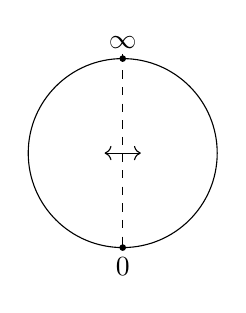
\begin{tikzpicture}[scale=0.6]
  % Draw the circle
  \draw (0,0) circle [radius=2cm];

  % Draw the points on top and bottom
  \coordinate (top) at (0,2);
  \coordinate (bottom) at (0,-2);
  \fill (top) circle [radius=2pt];
  \fill (bottom) circle [radius=2pt];

  % Draw the dashed arrow passing through the points
  \draw[dashed] (0,2.1) -- (0,-2.1);

  % Draw the horizontal arrows passing through the center
  \draw[<->, shorten >=2pt, shorten <=2pt] (-0.5,0) -- (0.5,0);

    % Add labels at the top and bottom
  \node[above] at (top) {$\infty$};
  \node[below] at (bottom) {$0$};
\end{tikzpicture}
\]
This is simply the circle with the $C_2$-action given by reflection across the equator. The two marked points are the only points fixed by the $C_2$-action.

We can also consider the regular representation $\rho$. This is a two dimensional representation, and so the underlying space is a 2-sphere. We can think of it as the one point complexification of $\mathbb{C}$, also known as $\mathbb{C}P^1$, equipped with the complex conjugation action. Since $\mathbb{R} \subseteq \mathbb{C}$ is fixed by conjugation, we see that $\mathbb{R}P^1 \subseteq \mathbb{C}P^1$ is fixed by this action. 
\[
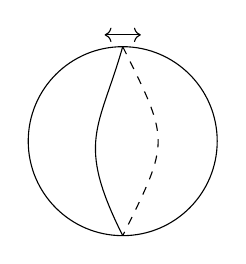
\begin{tikzpicture}[scale=0.6]
  % Draw the circle
  \draw (0,0) circle [radius=2cm];

    % Draw the points on top and bottom
  \coordinate (top) at (0,2);
  \coordinate (bottom) at (0,-2);

    % Define the control points to adjust the curve
  \coordinate (control1) at (-1,0);
    \coordinate (control3) at (-0.5,0.25);
  \coordinate (control2) at (1,0);

  % Draw the horizontal arrows passing through the center
  \draw[<->, shorten >=2pt, shorten <=2pt] (-0.5,2.25) -- (0.5,2.25);

    % Draw the curved lines
  \draw (top) .. controls (control3) and (control1) .. (bottom);
    \draw[dashed] (top) .. controls (control2) .. (bottom);
\end{tikzpicture}
\]
The  $C_2$-action is again given by reflection across an equator. 
\end{example}
\begin{notation}
Let $X$ and $Y$ be based spaces, then we let $\Map_G(X,Y) \subseteq \Map(X,Y)$ denote the space of $G$-equivariant maps $X \to Y$, with the subspace topology. Moreover, we can write define a $G$-space $G\Map(X,Y)$ to have underlying space $\Map(X,Y)$ with $G$-action given by 
\[
(g \cdot f)(x) \coloneqq g^{-1}f(gx). 
\]
The two are related: We have $G\Map(X,Y)^G = \Map_G(X,Y)$ as topological spaces, essentially by definition. 
\end{notation}
\begin{remark}
    Given a group homomorphism $H \to G$ we get a pullback functor $\phi^* \colon G\Top \to H\Top$ is the obvious way. For an injective homomorphism, this gives us restriction functors $\Res^G_H \colon G\Top \to H\Top$. This has a left and right adjoint, as we now explain. 
\end{remark}
\begin{definition}
    Let $X$ be a $H$-space, then we define a $G$-space $\Ind_H^G X = G \times_H X$ as the quotient of $G \times X$ by the relation $(g \cdot h, x) \sim (g, h \cdot x)$ for $g \in G, h \in H$. 
\end{definition}
\begin{example}
    If $H = e$ is the trivial group, then $\Ind_e^GX \cong G \times X$ is a free $G$-space. 
\end{example}
\begin{example}
    We have $\Ind_H^G(\ast) \cong G/H$. More generally, if $X$ is a space with trivial $H$-action, we have $\Ind_H^G(X) \cong X \times G/H$, where $G$ acts on $G/H$, and trivially on $X$. 
\end{example}
In analogy with Mackey functors, we have the following:
\begin{proposition}
    The functor $\Ind_H^G \colon H\Top \to G\Top$ is left adjoint to $\Res^G_H \colon G\Top \to H\Top$.
\end{proposition}
\begin{remark}
    There is a based version, which sends $X$ to $G_+ \wedge_HX $, the quotient of $G_+ \wedge X$ by the same relation as before. 
\end{remark}
\begin{remark}
    Similarly, there is a functor $\Coind_H^G \colon H\Top \to G\Top$, which sends $X$ to $\Map_H(G,X)$, the space of $H$-equivariant maps from $G$ to $X$, with $G$-action given by $(gf) \cdot g' = f(g \cdot g')$. This functor is right adjoint to restriction.

    In contrast to what we saw for Mackey functors, the left and right adjoint do not agree for spaces (Exercise: try and find an example). 
\end{remark}
\begin{remark}
    In fact, given $f \colon H \to G$ a group homomorphism, the pullback functor $f^* \colon G\Top \to H\Top$ always has a left and right adjoint. Taking $H$ to be the trivial group we can get functors called fixed points and orbits, which we now explicitly define. 
\end{remark}
\begin{definition}
    For $X \in G\Top$, the fixed points $X^G$ is the subspace
    \[
    X^G = \SET{x \in X}{g \cdot x = x \text{ for all } g \in G} \subseteq X.
    \]
This defines a functor $(-)^G \colon G\Top \to \Top$, which is right adjoint to pullback along $G \to e$. 
    
    More generally, we can define $X^H$ as the composite
    \[
    G\Top \xrightarrow{\Res^G_H} H\Top \xrightarrow{(-)^H} \Top.
    \]
\end{definition}
\begin{example}
    Returning to the representation spheres considered in Example~\eqref{ex:rep-spheres} we have $(S^{\sigma})^{C_2}  = S^0$, while $(S^{\rho})^{C_2} = S^1$. 
\end{example}
\begin{definition}
   For $X \in G\Top$, the orbit of a point $x \in X$ is the set 
   \[
   G \cdot x = \SET{g \cdot x}{g \in G}
   \]
   We can define an equivalence relation on $X$ by saying that $x \sim y$ if and only if there exists a $g \in G$ such that $g \cdot x = y$. The quotient by this equivalence relation is the orbit space $X/G$ of the action. This is the left adjoint of pullback along $G \to e$. 
\end{definition}
\begin{remark}
In summary: we have
\[
\Map_G(Y,X) \simeq \Map(Y,X^G)
\]
and
\[
\Map_G(X,Y) \cong \Map(X/G,Y)
\]
where $X$ is a $G$-space and $Y$ has the trivial $G$-action. 
\end{remark}
There is an obvious notion of homotopy in equivariant homotopy. 
\begin{definition}
    Two equivariant maps $f,g \colon X \to Y$ between $G$-spaces are said to be $G$-homotopic if there is an equivariant map $h \colon I \times X \to Y$ such that $h|_{\{ 0\} \times X} \simeq f$ and $h|_{\{ 1\} \times X} \simeq g$. Here we give $I$ the trivial $G$-action. 
\end{definition}
\begin{example}
    Let % https://q.uiver.app/#q=WzAsMixbMCwwLCJcXGFzdCJdLFsxLDAsIlNee1xcc2lnbWF9Il0sWzAsMSwiXFxpbmZ0eSIsMCx7Im9mZnNldCI6LTF9XSxbMCwxLCIwIiwyLHsib2Zmc2V0IjoxfV1d
$\begin{tikzcd}[ampersand replacement=\&]
	\ast \& {S^{\sigma}}
	\arrow["\infty", shift left, from=1-1, to=1-2]
	\arrow["0"', shift right, from=1-1, to=1-2]
\end{tikzcd}$  be the inclusion of the two fixed-points of $S^{\sigma}$. Because $S^{\infty}$ is path-connected, these are non-equivariantly homotopic. But they are not equivariantly homotopic, since the space of fixed points is not path-connected. 
\end{example}
We can now define $G$-homotopy groups, $G$-homotopy equivalences, etc. Note that by adjointness, the notion of equivariant homotopy will just be computing $\pi_n(X^G)$. Instead, it is better to remember the fixed points of all subgroups $H \le G$. To fix notation, let $\pi_n^H(X) \coloneqq \pi_n(X^H)$. 
\begin{definition}
    A morphism $f \colon X \to Y$ of $G$-spaces is a weak $G$-homotopy equivalence if the induced maps $\pi_n^H(f) \colon \pi_n^H(X) \to \pi_n^H(Y)$ are isomorphisms for all $H \le G$. 
\end{definition}
\begin{remark}
    By playing around with adjunctions we have $\pi_n^H(Y) = [G/H \times S^n,X]$, and so this leads naturally to the notion of $G$-CW-complex. 
\end{remark}
\begin{definition}
    A $G$-CW-complex is a sequential colimit of spaces $X_n$ where $X_{n+1}$ is a pushout (in $G\Top$)
% https://q.uiver.app/#q=WzAsNCxbMCwwLCJcXGNvcHJvZCBHL0ggXFx0aW1lcyBTXm4iXSxbMSwwLCJYX24iXSxbMCwxLCJcXGNvcHJvZCBHL0ggXFx0aW1lcyBEXm4iXSxbMSwxLCJYX3tuKzF9Il0sWzAsMV0sWzAsMl0sWzIsM10sWzEsM10sWzMsMCwiIiwxLHsic3R5bGUiOnsibmFtZSI6ImNvcm5lci1pbnZlcnNlIn19XV0=
\[\begin{tikzcd}[ampersand replacement=\&]
	{\coprod G/H \times S^n} \& {X_n} \\
	{\coprod G/H \times D^{n+1}} \& {X_{n+1}}
	\arrow[from=1-1, to=1-2]
	\arrow[from=1-1, to=2-1]
	\arrow[from=2-1, to=2-2]
	\arrow[from=1-2, to=2-2]
	\arrow["\ulcorner"{anchor=center, pos=0.125, rotate=180}, draw=none, from=2-2, to=1-1]
\end{tikzcd}\]
and $H$ ranges over all the subgroups of $G$. 
\end{definition}
\begin{example}
    We consider again the representation sphere $S^{\sigma}$. Here we start with the $C_2$-fixed 0-skeleton $S^0$. Here we attach a single free 1-cell $(C_2/e) \times D_1$ where one (free) endpoint is attached to 0 and the other to the point $\infty$. 
\end{example}
\section{The $G$-Whitehead theorem}
Our next goal is to prove the equivariant Whitehead theorem.
\begin{theorem}[Equivariant Whitehead theorem]
A weak $G$-homotopy equivalence between $G$-CW complexes is a $G$-homotopy equivalence. 
\end{theorem}
There are two ways to prove this theorem, both generalizing the two non-equivariant ways. The first is an inductive argument, and can be found in \cite[Theorem 2.1.31]{guillou}. The second is to prove a more general theorem, the equivariant homotopy extension and lifting property (HELP). The main subtly when extending the proof from the non-equivariant case is to define a suitable notion of the connectivity of a map. 
\begin{definition}
    Let $\theta \colon \Sub(G)/G \to \SET{x \in \bbZ}{x \ge -1}$. A map $f \colon X \to Y$ of $G$-spaces is $\theta$-connected if $f^H$ is $\theta(H)$-connected for all $H \le G$. A $G$-CW complex is $\theta$-dimensional if all cells of orbit type $G/H$ have non-equivariant dimension at most $\theta(H)$. 
\end{definition}
With these definitions in place, we now have an equivariant version of the HELP theorem.\footnote{For the details in the non-equivariant case, see \cite[Chapter 10.3]{May1999concise}.} 
\begin{proposition}
Let $A$, $X$, $Y$, and $Z$ be $G$-CW complexes such that $A \subseteq X$ is $\theta$-dimensional,
and let $e \colon Y \to Z$ be a $\theta$-connected $G$-map. Given $g \colon A \to Y$, $h \colon A \times I \to Z$, and $f \colon X \to Z$ such that $eg = hi_1$ and
$f|_A = hi_0$, there exist maps $\widetilde{g} \colon X \to Y$ and $\widetilde{h} \colon X \times I \to Z$ that make the following diagram commute:

% https://q.uiver.app/#q=WzAsOCxbMCwwLCJBIl0sWzIsMCwiQSBcXHRpbWVzIEkiXSxbNCwwLCJBIl0sWzAsMiwiWCJdLFsxLDEsIloiXSxbMiwyLCJYIFxcdGltZXMgSSJdLFs0LDIsIlgiXSxbMywxLCJZIl0sWzAsMSwiaV8wIl0sWzIsMSwiaV8xIiwyXSxbMCwzXSxbMyw0LCJmIiwyXSxbMSw0LCJoIiwyXSxbMSw1XSxbMyw1LCJpXzAiLDJdLFs2LDUsImlfMSJdLFsyLDZdLFsyLDcsImciXSxbNiw3LCJcXHRpbGRlIGciLDAseyJzdHlsZSI6eyJib2R5Ijp7Im5hbWUiOiJkYXNoZWQifX19XSxbNyw0LCJlIiwyLHsibGFiZWxfcG9zaXRpb24iOjMwfV0sWzUsNCwiXFx0aWxkZXtofSIsMix7InN0eWxlIjp7ImJvZHkiOnsibmFtZSI6ImRhc2hlZCJ9fX1dXQ==
\[\begin{tikzcd}[ampersand replacement=\&]
    A \&\& {A \times I} \&\& A \\
    \& Z \&\& Y \\
    X \&\& {X \times I} \&\& X
    \arrow["{i_0}", from=1-1, to=1-3]
    \arrow["{i_1}"', from=1-5, to=1-3]
    \arrow[from=1-1, to=3-1]
    \arrow["f"', from=3-1, to=2-2]
    \arrow["h"', from=1-3, to=2-2]
    \arrow[from=1-3, to=3-3]
    \arrow["{i_0}"', from=3-1, to=3-3]
    \arrow["{i_1}", from=3-5, to=3-3]
    \arrow[from=1-5, to=3-5]
    \arrow["g", from=1-5, to=2-4]
    \arrow["{\tilde g}", dashed, from=3-5, to=2-4]
    \arrow["e"'{pos=0.3}, from=2-4, to=2-2]
    \arrow["{\tilde{h}}"', dashed, from=3-3, to=2-2]
\end{tikzcd}\]
\end{proposition}
\begin{proof}[Sketch of proof]
The desired maps are constructed by induction on the skeleton of $X$, and then cell by cell, so we can assume that $X = G/H \times D^{n+1}$ and $A = G/H \times S^{n}$. By playing around with adjunctions, this reduces to the ordinary non-equivariant HELP theorem with $e \colon Y^H \to Z^H$, $X = D^n$ and $A = S^{n-1}$. 
\end{proof}
	% End the document without loading the bibliography
	% or the index, or the list of notation.
\end{document}